\begin{figure}[htbp]
    \centering
    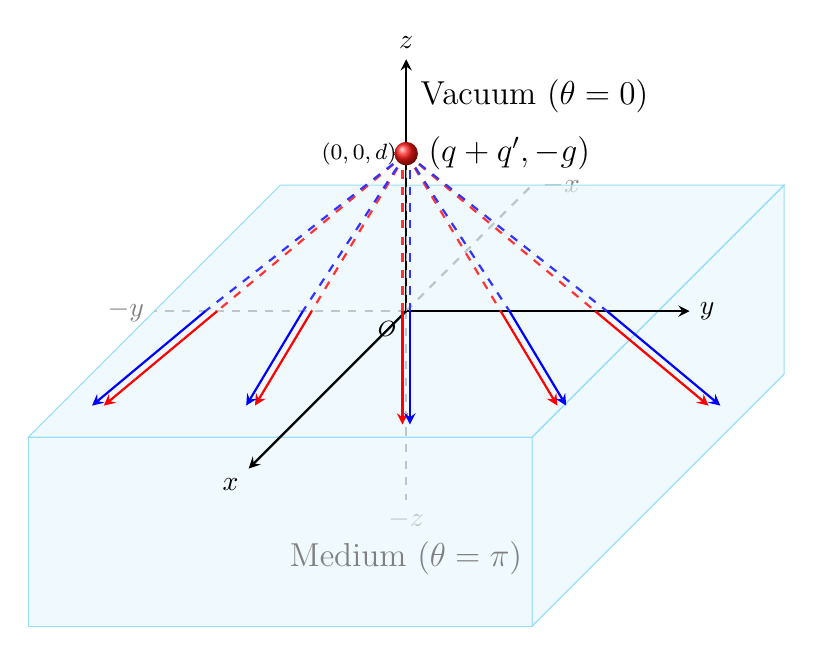
\begin{tikzpicture}[
        % 斜二测投影
        x={(-0.5cm, -0.5cm)}, 
        y={(1cm, 0cm)}, 
        z={(0cm, 1cm)}, 
        scale=0.8,
        axis/.style={->, thick, >=stealth, black},
        negaxis/.style={dashed, thick, gray},
        medium/.style={fill=cyan!10, fill opacity=0.6, draw=cyan!40, thin},
        charge/.style={shade, ball color=red!90, circle, inner sep=3pt},
        % 箭头样式:纯色,不透明
        rayRed/.style={->, >=stealth, thick, red, opacity=1},
        rayBlue/.style={->, >=stealth, thick, blue, opacity=1},
        dashRed/.style={dashed, thick, red!80},
        dashBlue/.style={dashed, thick, blue!80}
    ]
    
        % --- 参数定义 ---
        \def\limit{4}       % 平面半宽
        \def\slabH{3}       % 介质厚度
        \def\chargeH{2.5}   % 电荷高度 d
        
        % --- 1. 绘制内部/背景元素 (负坐标轴) ---
        \draw[negaxis] (0,0,0) -- (0,0,-\slabH) node[below] {$-z$};
        \draw[negaxis] (0,0,0) -- (-\limit,0,0) node[right] {$-x$};
        \draw[negaxis] (0,0,0) -- (0,-\limit,0) node[left] {$-y$};
    
    
        % --- 2. 绘制介质块 (背景) ---
        \filldraw[medium] (\limit, -\limit, 0) -- (\limit, \limit, 0) -- (\limit, \limit, -\slabH) -- (\limit, -\limit, -\slabH) -- cycle;
        \filldraw[medium] (\limit, \limit, 0) -- (-\limit, \limit, 0) -- (-\limit, \limit, -\slabH) -- (\limit, \limit, -\slabH) -- cycle;
        \filldraw[medium] (\limit, -\limit, 0) -- (\limit, \limit, 0) -- (-\limit, \limit, 0) -- (-\limit, -\limit, 0) -- cycle;
    
    
        % --- 3. 绘制正坐标轴 ---
        \draw[axis] (0,0,0) -- (\limit+1, 0, 0) node[anchor=north east] {$x$};
        \draw[axis] (0,0,0) -- (0, \limit+0.5, 0) node[anchor=west] {$y$};
        \draw[axis] (0,0,0) -- (0, 0, \limit) node[anchor=south] {$z$};
    
    
        % --- 4. 绘制新的场线结构 (Top Charge -> Medium) ---
        % 逻辑:从上方电荷发射,真空中为虚线,介质中为实线箭头
        
        \foreach \y in {-3, -1.5, 1.5, 3} {
            % 动态偏移量计算
            \pgfmathsetmacro{\len}{sqrt(\y*\y + \chargeH*\chargeH)}
            \pgfmathsetmacro{\gap}{0.12} 
            \pgfmathsetmacro{\yshift}{(\y > 0 ? 1 : -1) * \gap * \len / \chargeH}
    
            % --- 真空部分 (虚线) ---
            % 从电荷到界面点 (0, y, 0)
            \draw[dashRed] (0, 0, \chargeH) -- (0, \y, 0);
            \draw[dashBlue] (0, 0, \chargeH) -- (0, \y+\yshift, 0);
    
            % --- 介质部分 (实线箭头) ---
            % 从界面点向下延伸
            % 方向向量: (0, y, -d)
            \draw[rayRed] (0, \y, 0) -- ++(0, {0.6*\y}, {0.6*(-\chargeH)});
            \draw[rayBlue] (0, \y+\yshift, 0) -- ++(0, {0.6*\y}, {0.6*(-\chargeH)});
        }
        
        % --- Z轴方向的场线 ---
        \pgfmathsetmacro{\zGap}{0.06}
        % 真空 (虚线)
        \draw[dashRed] (0, -\zGap, \chargeH) -- (0, -\zGap, 0);
        \draw[dashBlue] (0, \zGap, \chargeH) -- (0, \zGap, 0);
        % 介质 (实线)
        \draw[rayRed] (0, -\zGap, 0) -- (0, -\zGap, -1.8);
        \draw[rayBlue] (0, \zGap, 0) -- (0, \zGap, -1.8);
    
    
        % --- 5. 绘制上方电荷与标注 ---
        \draw[dashed, thin, gray!80] (0,0,0) -- (0,0,\chargeH);
        
        \node[charge] (q) at (0,0,\chargeH) {};
        % 修改标注内容
        \node[anchor=west] at (0,0.2,\chargeH) {\large $(q+q', -g)$};
        \node[anchor=east] at (0,0,\chargeH) {\footnotesize $(0,0,d)$};
    
        % --- 6. 区域文字标注 ---
        \node[anchor=south east] at (-2, 3, 2) {\large Vacuum ($\theta=0$)};
        \node[anchor=north west, gray] at (4, 0, -1.5) {\large Medium ($\theta=\pi$)};
        \node[anchor=north east] at (0,0,0) {\footnotesize $O$};
    
    \end{tikzpicture}
    \caption{Mirage Monopole 2}
    \label{fig:mirage_monopole_2}
\end{figure}